
\documentclass[a4paper]{article}
\usepackage[utf8]{inputenc}
\usepackage[T1]{fontenc}     
\usepackage[francais]{babel}                        
\usepackage{tipa}
 \usepackage{textcomp}
\usepackage{graphicx}
\usepackage{array} % pour des tableaux particuliers                                                      
\usepackage[a4paper]{geometry}% Réduire les marges                         
\usepackage{multicol} % Pour faire plusieurs colonnes

	\usepackage{amssymb}
	\usepackage{mathrsfs}
	\usepackage{frcursive}
	\usepackage{color}

\usepackage{cite}
\usepackage[mediumspace,mediumqspace,Grey,squaren]{SIunits}

%\bibliographystyle{naturemag}



\title{L'apport des NGS pour inférer la structure de population}      
\author{Pierre-Louis STENGER$^{1}$}




\date{}                       % La date n\textquotesingleest pas requise (la date du jour de compilation est utilisé en son absence)

\sloppy                       % Ne pas faire déborder les lignes dans la marge

\usepackage{amsmath,amssymb,amsthm,amsfonts}
\usepackage{nicefrac}

\DeclareMathOperator{\reff}{}

 % % % % % % % % % % % % % % % % % % % MARGES  % % % % % % % % % % % %  % % % % % % % % % % % % % % 
 
\setlength{\hoffset}{-18pt}         
\setlength{\oddsidemargin}{0pt} % Marge gauche sur pages impaires
\setlength{\evensidemargin}{9pt} % Marge gauche sur pages paires
\setlength{\marginparwidth}{54pt} % Largeur de note dans la marge
\setlength{\textwidth}{481pt} % Largeur de la zone de texte (17cm)
\setlength{\voffset}{-18pt} % Bon pour DOS
\setlength{\marginparsep}{7pt} % SÈparation de la marge
\setlength{\topmargin}{0pt} % Pas de marge en haut
\setlength{\headheight}{13pt} % Haut de page
\setlength{\headsep}{10pt} % Entre le haut de page et le texte
\setlength{\footskip}{27pt} % Bas de page + sÈparation
\setlength{\textheight}{708pt} % Hauteur de la zone de texte (25cm)


 % % % % % % % % % % % % % % % % % % % FOND GRIS  % % % % % % % % % % % % % % % % % % % % % % % % % 

\usepackage{amssymb,amscd,latexsym,amsmath,amstext}
\usepackage{xkeyval}
\usepackage{framed}
\usepackage{xcolor}
\usepackage{fancybox}
\usepackage{multido}
\newlength{\DSFBox}
\newlength{\SSFBox}
\newlength{\DEFBox}
\newlength{\EFBox}
\makeatletter
\define@key{BCouleur}{ctexte}{\def\CTexte{#1}} % Couleur du texte
\define@key{BCouleur}{cbord}{\def\CBord{#1}} % Couleur du bord
\define@key{BCouleur}{cfond}{\def\CFond{#1}}   % Couleur du fond
\define@key{BCouleur}{sfbox}{\def\SFBox{#1}}        % pour \fboxsep
\define@key{BCouleur}{epaisfbox}{\def\EpaisFBox{#1}} % pour \fboxrule
% par dÈfaut
\setlength{\DSFBox}{5pt}
\setlength{\DEFBox}{3pt}
\setkeys{BCouleur}{ctexte=black,cbord=gray!20,cfond=gray!20,sfbox=\the\DSFBox,
epaisfbox=\the\DEFBox}{}
\newenvironment{BCouleur}[1][]{%
\setkeys{BCouleur}{#1}
  \def\FrameCommand{\fboxrule=\FrameRule \fboxsep=\FrameSep \color{\CTexte}\fcolorbox{\CBord}{\CFond}}
\setlength{\SSFBox}{\SFBox}
\setlength\FrameSep{\the\SSFBox}
  \setlength{\EFBox}{\EpaisFBox}
\setlength\FrameRule{\the\EFBox}
  \MakeFramed{\advance\hsize-\width \FrameRestore}}%
  {\endMakeFramed}
\makeatother

% % % % % % % % % % % % % % % % % % % % % % % % % % % % % % % % % % % % % % % % % % % % % % % % % 



\begin{document}
	
%\vspace*{\stretch{1}}
%\begin{cursive}
%\textbf{In the beginning there was nothing.
%\\
%God said: 'Let there be light !'
%\\
%There was still nothing, but now you could see it.
%\\
%(Dave Thomas)}
%\end{cursive}
%\vspace*{\stretch{1}}	
~~\\
~~\\
~~\\
~~\\
~~\\
~~\\
~~\\
~~\\
~~\\


\begin{center}
\Huge État de l'art
\end{center}

\newpage

\maketitle 

\large    
                                                   
$^{1}$Université de La Rochelle, Master 2 Gestion de l'Environnement et Ecologie Littorale (GEEL)

%\begin{BCouleur}  % Début fond gris

%\begin{abstract}
%Résumé
%\end{abstract}


%\end{BCouleur} % Fin fond gris
~~\\
\textbf{Mots clés:} \textit{NGS, Population, Génétique, Pyroséquençage, RAD-Seq, Illumina, MinION}
~~\\
%\section*{Introduction}   

Au cours du 20ème siècle, les avancées technologiques permettant d’accéder directement à l’\textbf{ADN (Acide Desoxyribonucléique)} et les nombreux progrès améliorant notre compréhension des mécanismes de l’\textbf{hérédité} ont posé les bases d’une nouvelle discipline : la \textbf{génomique} \cite{eggen2003approches}. 

La \textbf{séquence nucléotidique} (succession d'acides nucléiques qui composent l'ADN et qui est porteur de l'information génétique) permet dorénavant d'appréhender les variations phénotypiques (les différences de l'ensemble des caractères observables d'un individu) entre des êtres vivants \cite{champe1962reversal}.

L'objectif majeur de la génomique consiste à obtenir une connaissance et une compréhension de la structure et de la fonction des génomes (ensemble du matériel génétique d'un organisme) \cite{eggen2003approches}.

La diversité génétique est un concept central qui lie l'évolution biologique d'une espèce avec la complexité de l'organisme via son génome \cite{lynch2003origins}, le rétablissement de l'écosystème \cite{reusch2005ecosystem} et l'habilité des espèces à répondre aux changements environnementaux\cite{o1994role}.

En effet, selon \cite{lynch2003origins}, les séquences génomiques de diverses lignées phylogénétiques révèlent des augmentations importantes dans la complexité du génome de procaryotes par rapport aux eucaryotes. Ceci serait due à l'augmentation graduelle du nombre de gènes, résultant de la rétention de gènes en double, et des augmentations plus brusques de l'abondance des introns (parties de l'ADN non exprimées) et des éléments génétiques mobiles. \cite{lynch2003origins} soutiennent que le nombre de ces modifications est expliqué par des réductions à long terme la taille de la population.

En cas de résilience d'un écosystème suite à une pression, la \textbf{biodiversité} est expliquée par la complémentarité des génomes ("Genotypic complementarity") plutôt que par la sélection de génotypes particulièrement robustes \cite{reusch2005ecosystem}. Il est donc important de maintenir la diversité des espèces pour améliorer la résilience des écosystèmes dans un monde d'incertitudes croissantes environnementalement parlant \cite{reusch2005ecosystem}.

Les petites populations sont soumises aux risques de la \textbf{consanguinité}, de la \textbf{dérive génétique}, de la \textbf{perte de la variation génomique} globale due à la perte allélique, ou encore à la réduction de l'\textbf{hétérozygotie} (quand un individus possède deux allèles différents d'un même gène) \cite{o1994role}. Les conséquences de ces \textbf{déplétions génétiques} \cite{o1994role} peuvent être catastrophiques pour ces populations, voir pour l'espèce. Il est donc important d'appliquer les outils moléculaires de la génétique des populations pour la \textbf{conservation de ces espèces}.

Au sein des espèces, la \textbf{diversité génétique} est donc pensée pour refléter \textbf{la taille de la population, l'histoire, l'écologie et capacité d'adaptation.} 

De nombreuses techniques de biologie moléculaire existent pour obtenir ces informations. Pour ce faire, l'\textbf{ADN mitochondrial} (ADN provenant des mitochondries, et légué uniquement par la mère), les microsatellites (Séquences d'ADN formée par une répétition continue des mêmes bases) et l'\textbf{ADN nucléaire} (ADN provenant du noyau de la cellule) sont très utilisé. 

L'ADN mitochondrial semble être un marqueur de choix; il n' a généralement \textbf{pas de recombinaison}, a un \textbf{taux de dérive plus important} que l'ADN nucléaire et un niveau élevé de \textbf{polymorphisme} (propriété des espèces à se présenter sous plusieurs formes différentes) \cite{avise2000abandon}\cite{Aurelle:2009:aa}. 

Cependant, \cite{bazin2006population} montrent que l'ADN mitochondrial (ADNmt) est un marqueur couramment utilisé qui ne reflète pas l'abondance des espèces ou de l'écologie : la diversité de l'ADNmt n'est pas plus élevé chez les invertébrés que chez les vertébrés, en milieu marin que dans chez les espèces terrestres, ou que dans les petits organismes par rapport aux grands. Le loci nucléaire (ADN nucléaire), en revanche, est adapté à ces attentes intuitives. La distribution inattendue de la diversité mitochondrial est expliquée par l'\textbf{évolution adaptative récurrente} (évolution répétée d'un caractère particulier), contestant la \textbf{théorie neutraliste de l'évolution} (selon laquelle la plupart des mutations ont une influence négligeable sur la fitness (succès reproducteur) de l'individu, et ne donne donc qu'une influence ponctuelle à la sélection naturelle) et de remettre en question la pertinence de l'ADNmt dans les études de la biodiversité et de conservation; ce qui correspond à environ trente ans de recherche scientifique (communication personnelle, Benoit Simon-Bouhet). Malgré tout, ce marqueur permet de fournir une première image de la structuration génétique d'une espèce \cite{Aurelle:2009:aa}. De plus, \cite{kitchen2008three} ont démontré une corrélation positive entre l'ADNmt et les variations des allozymes, ce qui suggère que la diversité de l'ADNmt peut corréler avec la taille de la population.

Néanmoins, \cite{kashi2006simple} remettent aussi en cause l'utilisation des \textbf{microsatellites}, ainsi que l'hypothèse d'une évolution neutre des marqueurs employés \cite{Aurelle:2009:aa}. Les microsatellites, en vertu de leurs qualités de mutations et de leurs qualités fonctionnelles, jouent un rôle majeur dans la génération de la variation génétique impliquant une évolution adaptative \cite{kashi2006simple}.

Depuis le début des \textbf{années 2000}, de nouvelles technologies apparaissent, permettant de répondre aux questions de la génétique des populations, en limitant les coûts, le temps et les biais. Le \textbf{séquençage} (qui permet la détermination de la séquence des gènes) haut débit, appelé \textbf{NGS} pour \textbf{Next-Generation Sequencing}, a radicalement changé le paysage de la génomique, et pour inférer la structure de population.

\begin{figure}[!h]
\centering{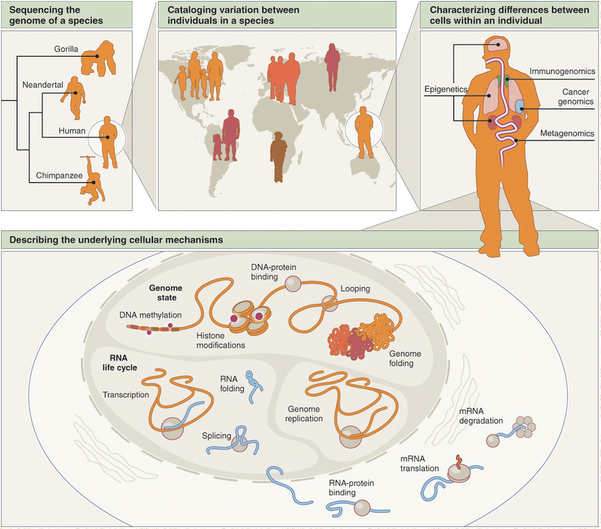
\includegraphics[scale=0.5]{shendure}}
\caption{Les NGS permettent de travailler à différentes échelles\cite{shendure2012expanding}}
\end{figure}

En effet, les méthodes traditionnelles en génétiques des populations ne mettaient en lumière que les effets de la \textbf{dérive génétique} (fixation d'un allèle (une des versions différentes d'un même gène) dans la population), les \textbf{mutations} et les \textbf{migrations}. Mais c'est l'avènement des NGS qui a permis de prendre en compte les effets de la sélection, mais aussi à \cite{bazin2006population} et à \cite{kashi2006simple} de remettre en question ces anciennes pratiques. 

De nouvelles formes de NGS apparaissent rapidement, baissant toujours plus les coûts et les temps de séquençage. Cette évolution est encore plus rapide que la conjecture (loi) de Moore (voir figure \ref{moore}), en effet, en dix ans, le prix d'un séquençage a été divisé par 100 000.

\begin{figure}[!h]
\centering{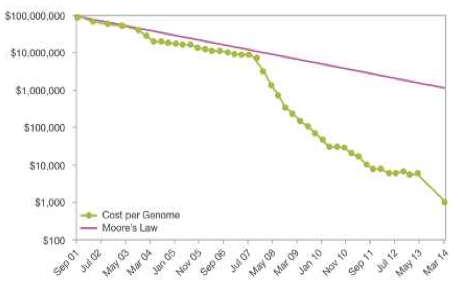
\includegraphics[scale=0.5]{evolution}}
\caption{Evolution très rapide des instruments, des débits et des coûts (premier séquençage sur 454 en Janvier 2008)\label{moore}}
\end{figure}

La qualité et la quantité des résultats a donc explosé. Avec la \textbf{technique Sanger} (première technique de séquençage ADN, en 1977 par Frédérick Sanger) 96 ADNs différents pouvaient être analysés en une fois, alors qu'avec les NGS ce sont des millions d'ADNS différents qui peuvent être analysés en une fois. C'est un véritable saut technologique.

Il existe de nombreuses technologies et plateformes dont les principales sont la technique de \textbf{pyroséquençage 454} (Société Roche, avec les appareils GS Junior System, et GS FLX+ System), la technique d'\textbf{Illumina} (Société Solexa avec les appareils HiSeq System, Genome analyser Ilx ou encore MySeq), la technique  \textbf{Applied Biosystems} de Life Technologies avec les appareils SOLID 5500 System ou encore la technique \textbf{Ion Torrent} de la même société (Life Technologies, avec les appareils Personal Genome Machine et Proton). À partir de 2012, une nouvelle génération de séquenceur encore plus performant arrive sur le marché, appelé "troisième génération de séquenceur" ou encore "\textbf{Next-Next Generation Sequencing}". Les principales techniques sont celles d'\textbf{Helicos} (avec l'appareil Helicos Genetic Analysis System), la technique \textbf{Pacific Biosciences} avec PacBio RS ou encore la technique d'\textbf{Oxford Nanopore Technologies} avec GridION System et MinION. 

Il ne sera présenté ici que la technique de pyroséquençage 454, la technique d'Illumina via la technique RAD-Seq et la technique d'Oxford Nanopore via le MinION.

Toutes ces NGS se basent sur le même principe. Il faut \textbf{fragmenter} l'ADN, créer des \textbf{banques d'ADN} par ligation d'adaptateurs, les \textbf{cloner} (soit par PCR en émulsion sur une bille dans des microréacteurs (décrit plus bas, dans la technique 454) comme pour les techniques 454 ou SOLID, ou alors par "Bridge" PCR (Polymerase Chain Reaction) sur un support plan (Flow cell) ce qui permet de créer des colonies d'ADn se nommant polonies, comme dans la technique Illumina), puis ces clones sont \textbf{séquencés} par une des techniques vu précedemment. Par réaction chimique, de la luminescence est émise (décrit plus bas, dans la technique 454) ce qui permet de convertir les séquences en fichier informatique.

%\subsection{Le pyroséquençage, exemple de la technique 454}
~~\\

En 2005, Jonathan M. Rothberg a élaboré la technologie de \textbf{pyroséquençage 454} Life Sciences (depuis racheté par Roche) et a prouvé la robustesse de ce séquençage en séquençant le génome de \textit{Mycoplasma génitalium} \cite{Margulies:2005aa} et qui ne nécessite pas de clonage (donc gain de temps et d’argent), et permet une lecture directe de la séquence obtenue après le séquençage.\cite{sengenes2012developpement}.

La particularité de cette technologie est qu'elle repose sur trois phases, dont une phase centrale de PCR en émulsion pour l'amplification des fragments à séquencer. \cite{Margulies:2005aa} \cite{sengenes2012developpement}

La première phase correspond à la \textbf{préparation de la banque:} L’ADN que l'on souhaite séquencer est dans un premier temps fragmenté par nébulisation \cite{loman2012performance} (pour les petits ADN de \unit{0.5-5}{\micro\metre}\cite{Prodromou:2007aa}, et utilisé avec de l'azote comprimé)\cite{syed2009next} , par audition hydrodynamique \cite{poptsova2014non} (pour les ADN de taille moyenne \unit{5-10}{\micro\metre})\cite{Prodromou:2007aa} qui est obtenu à l'aide de pressions aquatiques exercées sur les molécules d'ADN \cite{poptsova2014non} ou par "sonication" \cite{Knierim:2011aa} (pour les gros ADN de \unit{10-100}{\micro\metre})\cite{Prodromou:2007aa} où les échantillons sont soumis à des ondes ultrasonores, dont les vibrations produisent des cavitations gazeuses dans le liquide qui cisaillement les molécules d'ADN par vibration de résonance \cite{Knierim:2011aa}. afin d'obtenir des fragments d'environ 300pb. Les extrémités cohésives créent lors de la coupure vont être réparées afin d’obtenir des extrémités franches permettant l’ajout des adaptateurs.\cite{Prodromou:2007aa} \cite{sengenes2012developpement}

Par le biais d'une ADN ligase \cite{sengenes2012developpement}, on ajoute ensuite des adaptateurs qui contiennent notamment une séquence MID (Multipled IDentifier) qui permettra d'identifier chaque échantillon lors du séquençage. \cite{Margulies:2005aa}

La seconde phase est l'\textbf{amplification clonale par PCR (Polymerase Chain Reaction) en émulsion (emPCR):}

La PCR à lieu dans une microgoutte avec une microbille d'agarose en phase aqueuse, baignant dans de l'huile avec plusieurs autres millions de billes. Chaque bille comprend donc plusieurs copies d'un même brin d'ADN. Chacune des billes est disposée dans un des 1,6 millions de puits d'un support nommé PTP (PicoTiterPlate) \cite{sengenes2012developpement}

La dernière phase correspond à la \textbf{réaction de séquençage en elle même qui est le pyroséquençage:} ces réactions se produisent dans chaque puits avec les nucléotides qui traversent l'un après l'autre la PTP (voir figure \ref{1}). Quand la polymérase incorpore un nucléotide, un pyrophosphate (PPi) est alors libéré, et par le biais de cascades enzymatiques, une adénosine triphosphate (ATP) est crée qui va ensuite convertir la luciférine en oxyluciférine via une luciférase. C'est cette dernière réaction qui produit de la lumière, et plus de nucléotides seront incorporés, plus la réponse lumineuse sera importante. Ces signaux lumineux sont captés par la machine qui les convertis en information numérique. \cite{sengenes2012developpement}

Cette technique présente malgrè tout des limitations:

\begin{itemize}
\item \textbf{Pour l'extraction des données:} un fichier SFF (Standard Flowgram File) est créé en sortie standard du 454 (Fichier binaire qui est humainement illisible\cite{Peyretaillade:2010}), pour le lire il faut un exécutable fourni par la société Roche (sffinfo, uniquement pour ordinateurs avec noyeau Unix (Linux, iOs...))
\item \textbf{Les erreurs de séquençage peuvent être nombreuses:} 

\begin{enumerate}
	\item Il existe des {\itshape insertions ou des délétions} qui rendent difficile à déterminer le nombre de nucléotides entrant dans la composition d'un homopolymère (suite d'un même nucléotide), possible perte de la relation de linéarité entre l'intensité lumineuse émise et le nombre de nucléotides incorporé \cite{Peyretaillade:2010}. Il peut aussi y avoir détection d'un signal provenant d'un puits adajacent \cite{Peyretaillade:2010}. Selon \cite{balzer2011systematic}, le \textbf{phénomène de CAFIE} (CArry Forward/incomplete Extension) est une erreur de séquençage (qui rend les séquences incomplètes) relativement commune.
	\item Des {\itshape bases ambigües} peuvent apparaitre dans la séquence sous forme de code particulier (par exemple un "N" correspond à une base inconnue, ou encore un Y correspond à une hésitation entre les bases C et T...(Communication personnelle; Amélia Viricel-Pante)) 
	\item Des {\itshape erreurs de prédiction} sont aussi possible comme un signal surestimé suivi d'un signal sous-estimé ou vice versa. \cite{gilles2011accuracy}
	\end{enumerate}

\item \textbf{Par des réplicas artificiels:} ils correspond 4 à 44 pourcents des erreurs selon \cite{niu2010artificial} et 11 à 35 pourcents selon \cite{gomez2009systematic}). Il y a plusieurs billes dans une même goutte d’émulsion dont une seule porte un fragment d’ADN. La caméra détecte une émission de lumière dans un ou plusieurs puits vides provenant d’un puits adjacent où s’effectue la réaction de pyroséquençage \cite{Peyretaillade:2010}.
\item Et enfin il existe des \textbf{séquences chimériques (amplicons)}, qui sont des séquences qui se sont hybridées\cite{haas2011chimeric}.
\end{itemize}

En 2005, Rothberg annonça que cette technologie permettrait de séquencer le génome de James D. Watson pour seulement 1 millions de dollars \cite{Margulies:2005aa} \cite{sengenes2012developpement}.
Ils réussirent en 2007 en respectant le budget annoncé, et en le réalisant en deux mois \cite{wheeler2008complete}. En 2006, c'est avec cette technique que le génome de l'homme de Néanderthal à pu être séquencé \cite{green2006analysis}, \cite{noonan2006sequencing}, même si \cite{Wall:2007aa} ont démontré qu'il y avait majoritairement de l'ADN humain moderne contaminant \cite{sengenes2012developpement}.

\begin{figure}[!h]
\centering{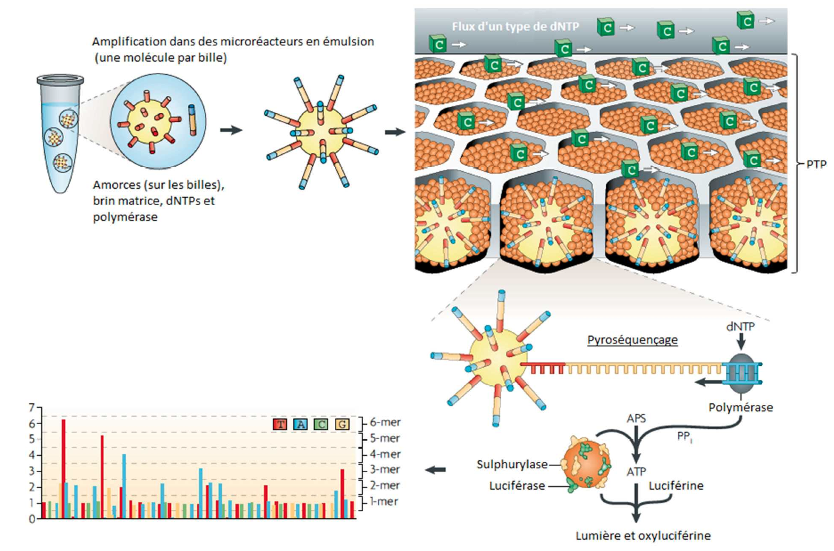
\includegraphics[scale=0.5]{454totale}}
\caption{Aperçu de la technologie 454 \cite{sengenes2012developpement}, PTP: PicoTiter Plate, PPi: pyrophosphate inorganique, APS: adénosine phosphosulphate, ATP: adénosine triphosphate.\label{1}}
\end{figure}

%\subsection{RAD Seq}
~~\\

Les \textbf{marqueurs des sites de restriction} (séquence particulière de nucléotides qui est reconnue par une enzyme de restriction comme un site de coupure dans la molécule d'ADN) associés à l'ADN (\textbf{RAD-Seq}: Restriction site Associated DNA) sont utilisés pour la cartographie génétique, dont la cartographie des QTL (Quantitative Trait Loci), mais aussi dans la génétique des populations, et donc dans la compréhension de l'évolution \cite{davey2010radseq}. 

\begin{figure}[!h]
\centering{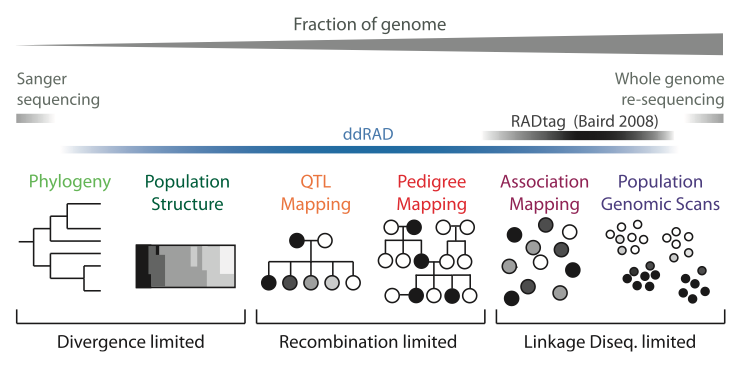
\includegraphics[scale=0.5]{genscan}}
\caption{Résolution des marqueurs de type RAD: Un procédé de génotypage souple peut être utilisé pour optimiser le nombre de marqueurs génétiques pour une approche expérimentale spécifique dans un système biologique donné\cite{peterson2012double}}
\end{figure}

La \textbf{technique RAD-Seq} est un séquençage de type NGS qui lie les séquences aux sites de restriction \cite{Baird:2008aa}, puis fragmente le génome par digestion enzymatique, réalise des ligation d'amorces et un code barre (pour distinguer les différents échantillons \cite{davey2013special}). Il faut isoler les balises RAD (\textbf{RAD-tags}), puis les séquences ADN flanquent immédiatement dans chaque site de restriction dans tout le génome. Il y a donc deux fois plus de RAD-tags que de sites de restriction\cite{davey2013special}. Une fois les balises RAD isolées, on identifie et recherche les SNP (Single Nucleotide Polymorphism) pour voir le polymorphisme \cite{hohenlohe2010population}. Il est utilisé sur des séquenceurs de type Illumina, SOLID ou encore Ion Torrent PGM \cite{hohenlohe2010population}. 

\begin{figure}[!h]
\centering{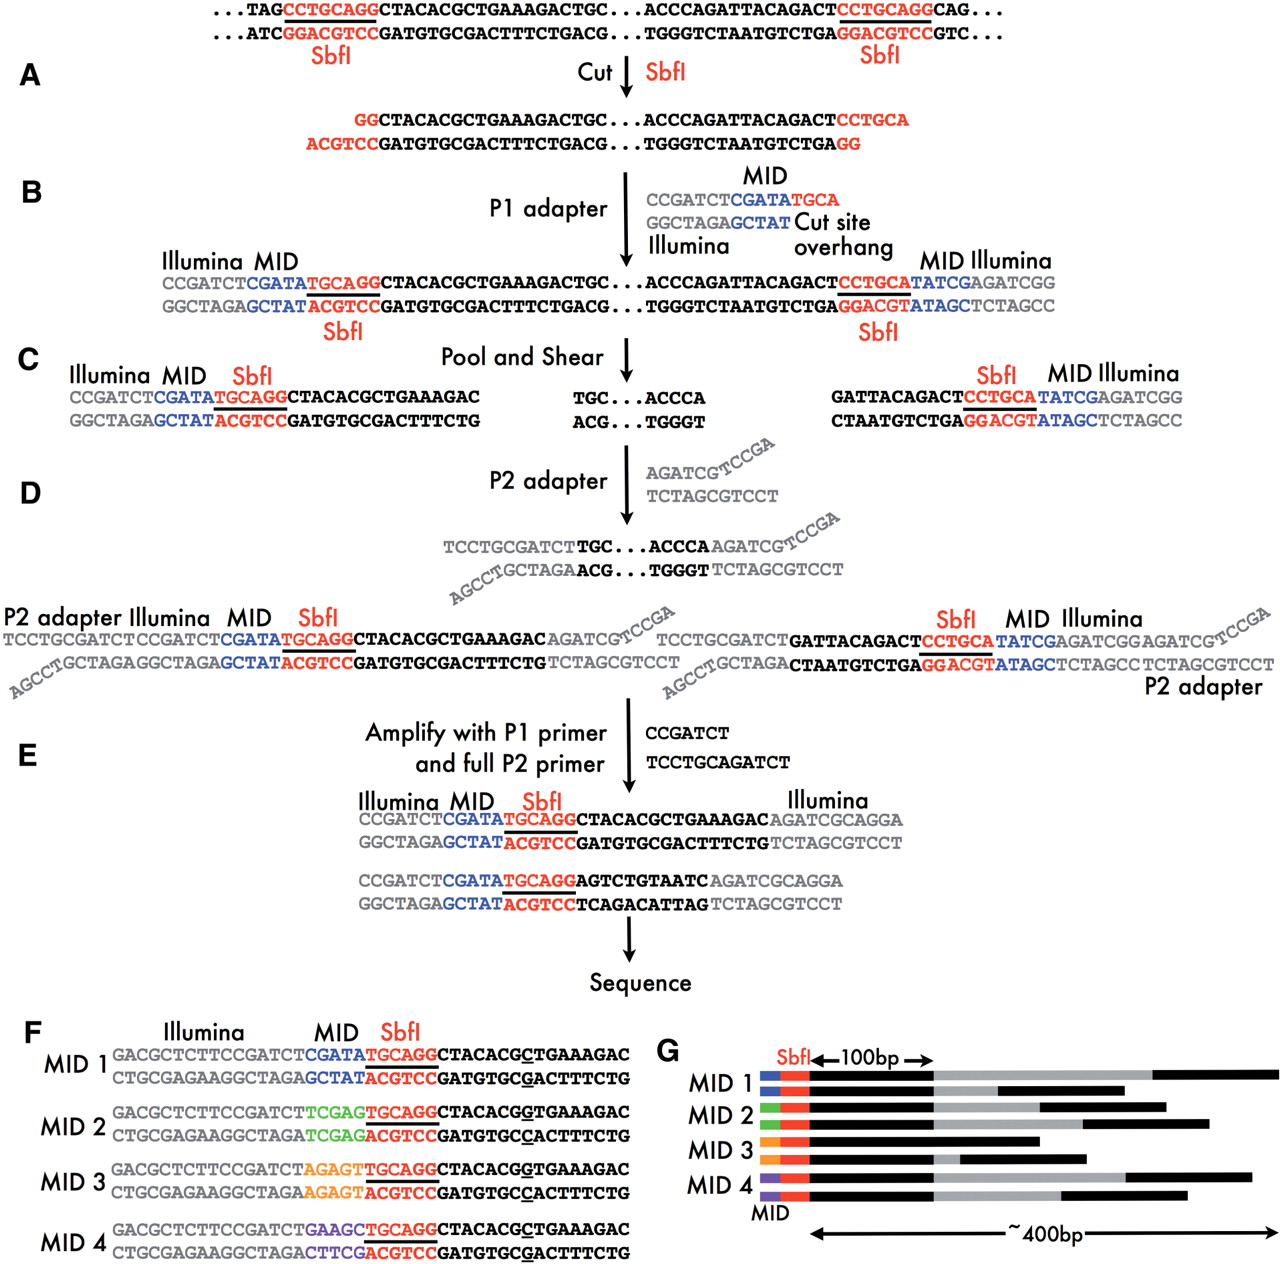
\includegraphics[scale=0.25]{radseq}}
\caption{Étapes pour obtenir des séquences d'ADN via la technique Rad seq}
\end{figure}

C'est une technique très utilisée pour la \textbf{biologie évolutive}:

\begin{itemize}
\item \cite{hohenlohe2010population} ont utilisé la \textbf{technique Illumina-sequenced RAD tags} pour identifier plus de 45 000 SNP chez 100 épinoches (\textit{Gasterosteus aculeatus}) provenant de la mer ou de rivières. Cette étude est une première en terme \textbf{scannage génomique} de haute densité basé sur des SNP permettant de calculer la diversité génétique et la différenciation de ces populations d'épinoches dans la nature. Ceci a permit de d'identifier les régions génomiques, d'élucider la part évolutive et démographique de ces populations naturelles et donc de trouver \textbf{des gènes candidats de signification évolutive}. 

\item De la \textbf{cartographie à l'aide de marqueurs} a était réalisé sur des Lepisosteus (\textit{Lepisosteus oculatus})\cite{Amores:2011aa}, ce qui a permit de découvrir que c'est une lignée de poissons qui a divergée avant la duplication du génome des téléostéens (ce qui correspond à un "Outgroup"). De plus, cette technique a mis en lumière que leur génome est plus proche de celui des hommes que celui des autres téléostéens (voir figure \ref{2}).

\begin{figure}[!h]
\centering{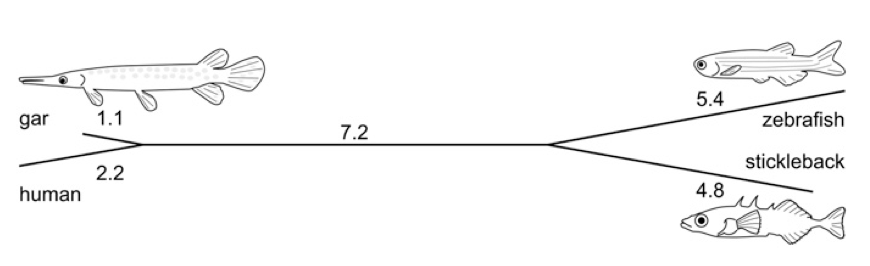
\includegraphics[scale=0.5]{teleo}}
\caption{Comparaison synthetique de deux téléostéens (zebrafish and stickleback) par rapport au lepisosteus et à l'homme. La longueur des branches est proportionnelle à l'estimation du nombre de divergence en terme de chromosome entre les espèces \cite{Amores:2011aa}\label{2}.}
\end{figure}


\item Les \textbf{scans génomiques} sur des milliers de SNP peuvent permettre de découvrir un patron de divergence et/ou un flux de gènes entre des espèces écologiquement divergente, comme pour \textit{Populus tremula} avec \textit{Populus trichocarpa} \cite{Stolting:2013aa}. Stölting et ses collègues ont scanné le génome de ces deux arbres hybrides différents d'un point de vue écologique. Ils ont utilisé plus de 38 000 SNP en utilisant la méthode de RAD-seq et ils ont découvert une grande divergence génétique (e.g. la proportion de SNP fixé) entre les espèces sur 11 des 19 chromosomes. Ceci correspondrait plus à un flux de gènes régulier qu'a du polymorphisme ancestral partagé. Ces résultats permettent donc d'expliquer l'origine de ces "génomes mosaïques" \cite{Stolting:2013aa} vu dans ces taxa avec des génomes dits "poreux" \cite{Stolting:2013aa} et suggèrent une introgression ou une conservation extensive naissante parmis les espèces des chromosomes sexuels chez ces végétaux. 

\item Le RAD-seq permet aussi de réaliser de la \textbf{phylogéographie}. En effet, un nombre très large de SNP à travers le génome a le pouvoir d'affiner nos connaissances sur l'histoire démographique d'une population et d'identifier les régions du génome où la sélection naturelle a agit. \cite{Reitzel:2013aa} ont utilisé cette technique sur une anémone américaine (\textit{Nematostella vectensis}) en guise de modèle. Des centaines de SNP contenant des "tags" ont été identifiés dans des milliers de RAD loci provenant de 30 individus barcodés de quatre lieux différents sur la côte Est des Etats-Unis d'Amérique. Malgré le manque d'information sur cet espèce (e.g. de génome de référence), un arbre phylogénétique a pu être créé (voir figure \ref{3}) \cite{Reitzel:2013aa}.

\begin{figure}[!h]
\centering{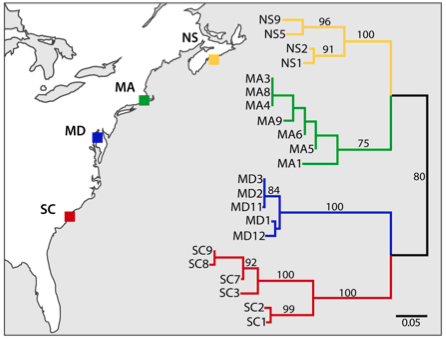
\includegraphics[scale=0.5]{geo}}
\caption{Phylogéographie de \textit{N. vectensis}: Nova Scotia (NS), Massachusetts (MA), Maryland (MD), and South Carolina (SC) \cite{Reitzel:2013aa}\label{3}.}
\end{figure}

\item La \textbf{phylogénomique} a vu ses capacités augmenter grâce à la technique RAD-seq. L'analyse des bibliothèques RAD en utilisant des outils bioinformatiques et phylogénétique a permit d'avoir 400 fois plus de sites que l'approche de Sanger et d'avoir par exemple une phylogénie basée sur un alignement de 2 262 825 nucléotides par espèces chez des coléoptères \cite{cruaud2014empirical}. Ainsi les relations entre 18 espèces de carabes qui ont divergé il y a 17 millions d'années ont pu être déterminés avec précision \cite{cruaud2014empirical}, alors que les techniques de Sanger via l'ADN nucléaire et mitochondrial ne donnaient pas les mêmes résultats (voir figure \ref{4}). 

\begin{figure}[!h]
\centering{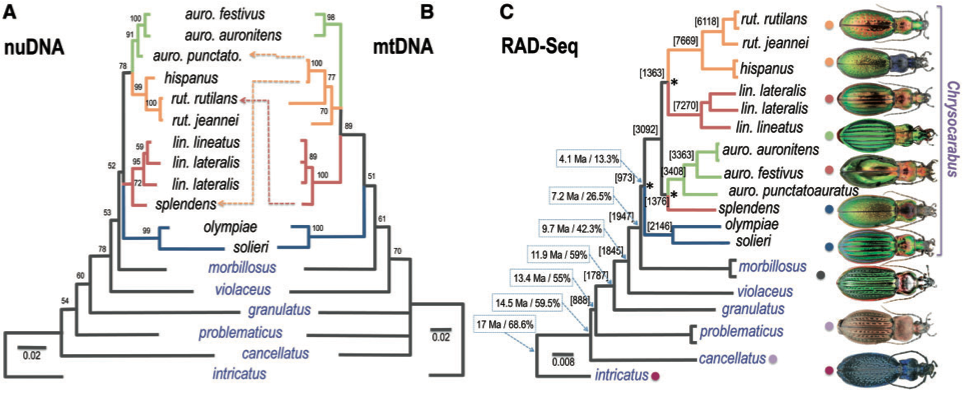
\includegraphics[scale=0.5]{carabe}}
\caption{Phylogénie des carabes obtenues par ADN nucléaire (A), ADN mitochondrial (B) et via la technique de RAD-Seq (C)\cite{cruaud2014empirical} \label{4}.}
\end{figure}

\item C'est aussi une technique très utilisé pour la \textbf{délimitation d'espèces} \cite{herrera2015rad}\cite{Pante:2015aa} et la \textbf{structure des populations} \cite{Pante:2015aa}. Selon les techniques classiques de génétiques, les \textit{Chrysogorgia} sont des coraux profonds dont les espèces sont délimitées par un seul haplotype mitochondrial \cite{herrera2015rad}\cite{Pante:2015aa}. Avec la technique de RAD-Seq le nombre de loci homologues RAD à décru dramatiquement  avec une baisse de la divergence. Plus de 70 pourcents des loci étaient perdus lors de la comparaison de spécimens séparés par deux mutations sur un brin mitochondrial de 700 nucléotides. Ainsi, six espèces sur neuf ont été confirmées, et il se peut que des individus caractérisé par un même haplotype mitochondrial peuvent appartenir à des espèces disctinctes. À l'inverse, trois haplotypes mitochondriaux forment un clade bien supporté dans lequel aucune structure de population n'a été détecté, ce qui suggère une possible variation intraspécifique de l'ADN mitochondrial chez \textit{Chrysogorgia}. Ainsi, les données RAD ont permis à peaufiner les interprétations des marqueurs mitochondriaux classiques utilisés dans les octocoraux pour délimiter les espèces et de découvrir la diversité détectée auparavant \cite{Pante:2015aa}.

\end{itemize}

Il existe cependant quelques difficultés liées au génotypage de SNPs RAD-tags \cite{Pante.E.:2014} \cite{mastretta2015restriction}.
En effet, \textbf{en laboratoire}, la qualité des réactifs peut-être hétérogène, les risques de contamination sont possible, des erreurs de pipetage peuvent subvenir, la sensibilité de l’enzyme à la qualité de l’ADN n'est pas toujours la même, ou encore des biais liés aux PCR. \cite{Bonin:2004aa}, \cite{Baird:2008aa}, \cite{peterson2012double}, \cite{hohenlohe2012extensive}, \cite{Pante.E.:2014}
De plus, il peut y avoir des erreurs \textbf{de séquençage} ou encore un séquençage aléatoire d’allèles et de loci \cite{meacham2011identification}, \cite{nielsen2011genotype}, \cite{hohenlohe2012extensive}, \cite{loman2012performance}, \cite{Pante.E.:2014}.
Il peut aussi y avoir des erreurs \textbf{intrinsèques au génome} comme le polymorphisme sur les sites de restriction ou la méthylation du site de restriction \cite{davey2013special}, \cite{gautier2013effect}, \cite{Pante.E.:2014}.

~~\\

Les \textbf{techniques de Next-Next generation sequencing} qui ont vu le jour en 2012 permettent un séquençage sur une molécule unique et de ce passer de l'amplification clonale \cite{Boyle:2014:aa}. Cependant, le taux d'erreur de séquençage est 10 fois plus élevé qu'avec le séquençage de type Sanger \cite{Boyle:2014:aa}. L'appareil \textbf{MinION} (voir figure \ref{minion}) d'\textbf{Oxford Nanopore Technologies} "deviendra l'approche par défaut du séquençage d'ADN circulaire pour étudier la variété des espèces" selon \cite{hargreaves2015assessing}. 

Le MinION est un dispositif portable pour les analyses moléculaires grâce à la technologie nanopore. Il est adaptable pour l'analyse de l'ADN, de l'ARN, des protéines ou de petites molécules avec un flux de production simple \cite{nanoport}.

Le principe de la technologie nanopore consiste à faire passer l'ADN le long d'un pore qui est formé par une première protéine qui permet de séparer les deux brins d'ADN (voir figure \ref{nano}) \cite{Boyle:2014:aa}. Puis le passage de l'ADN simple brin au sein de la seconde protéine provoque un \textbf{courant électrique} caractéristique de chaque base de l'ADN \cite{Boyle:2014:aa}. Ce courant électrique et ensuite traduit en information numérique \cite{hargreaves2015assessing}. 

Cet appareil à déjà fait ses preuves, notamment pour séquencer rapidement les ARN et ADN de pathogènes comme celui du virus Ebola, donnant des informations scientifiques et sur la santé publique en un temps record \cite{Hoenen:2015:aa} mais aussi pour réaliser de la taxonomie microbienne de haute résolution et en même temps dans diverses analyses de diversité microbienne via l'étude de l'ADN 16S \cite{benitez2015species}. Ou encore pour la détection en temps réel des gènes de résistance aux antibiotiques, par exemple en cas de pic de Salmonelles dans un hôpital \cite{Quick:2015aa}.

\begin{figure}[!h]
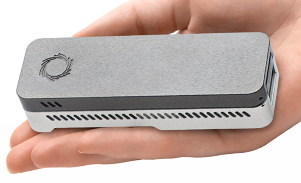
\includegraphics[scale=0.75]{Nanoport} \hfill
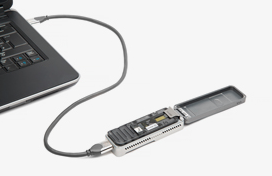
\includegraphics[scale=0.75]{Nanoport2}
\caption{Le MinION \label{minion}}
\end{figure}

\begin{figure}[!h]
\centering{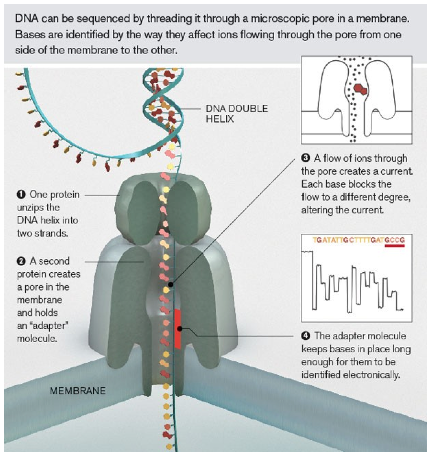
\includegraphics[scale=0.5]{nano}}
\caption{Séquençage de l'ADN via Nanopore\label{nano}}
\end{figure}


%PredRAD: \cite{herrera2014genome} fréquence des sites de coupe extrêmement variable,
%dépend des groupes taxinomiques
%plus le site de coupe est long, moins les sites de coupes sont fréquents sur le génome pas de corrélation claire entre composition en nt du site de coupe et sa prévalence
%prévalence de certains tri-nucléotides meilleur indicateur de fréquence de sites de coupe



%RAD sequencing enables unprecedented phylogenetic resolution and objective species delimitation in recalcitrant divergent taxa \cite{herrera2015rad}

%Conclusions:

%RAD-tag, une représentation réduite du génome
%couplage enzyme de restriction / NGS
%large panel d’utilisations (cartographie -> phylogénétique)
%déclinaisons (e.g. ddRAD) augmentent l’applicabilité
%‣
%compromis rendement / mise en oeuvre / échelle (échantillonnage, phylogénétique...)

%large panel d’outils / pipelines bioinformatiques 

%outils diffèrent par leur stratégies de détection des loci, polymorphisms, allèles

%détection nécessaire des erreurs liés à ces détections (locus drop-out, allele drop-out, genotyping error...)
%‣
%compromis nb marqueurs / taux d’erreur

%stratégies de mise en oeuvre en laboratoire
%--> choix du nb d’individus, de l’enzyme, de la plateforme de séquençage, du nb de runs...
%--> réplicats techniques: individus / banques / séquençage 

%stratégies de traitement bioinformatique des données
%--> choix de la plateforme de traitement, philosophie des outils disponibles (e.g. Stacks vs. PyRAD)
%--> exploration de l’espace paramétrique (e.g. couverture, divergence) et estimation de l’incertitude liée au génotypage




%\section{Mémo notes}

%Apport des NGS pour inférer la structure de population

%--> Qu'est ce que ça nous apprend de plus ?

%Méthodes traditionnelles en génétiques des populations --> Dérive, mutation et migration. --> "On était bien" BSB\copyright

%NGS ont permis de prendre en compte la sélection et ça à mis 30 ans de recherches en question.

%~Basin (2006) --> Taille de la population décorrélé au nombre de diversité mitochondriale --> Il faudrait faire un balayage sélectif
%~~\\
% RAD SEQ --> Moins de marqueur que 454
%Amélia --> Dauphin commun --> Structure population en Atlantique --> Augmentation du nombre de marqueur --> Augmentation de la puissance statistique
%Car génétique ne montrait qu'une seule population, alors que écotoxicologie et isotopes en montraient plusieurs.
%On va travailler sur marqueur de sélection --> Adaptation locale --> Ce sont les marqueurs Outlayer --> FST --> Avec les FST on revient dans un système circulaire (on a deux populations, on veut les différencier, on a un FST, on regarde si c'est supérieur. Aurait-on le même résultats avec 5 population ? Si on a 1000 marqueurs, il y en a forcement --> Statistiques fréquentistes (c'est à l'opposé des statistiques bayésiennes))
%--> On coupe le jeu de données en deux.
%~~\\
%Do it yourself ABC (Marie Louis, usé à la fin de thèse)
%--> Histoire évolutive
%~~\\
%Eric: 
%\begin{itemize}
%\item Séquenceur nanoport (Oxford)
%\item Micness --> Séquence en NGS les microsatelites, Marie Suez et al. 2015
%\end{itemize}

% Séquenceur à plaques --> N'est pas un NGS

% Génome scan 
% Familles de méthodes (pyroseq, rad seq, ce qui est produit par genome scan)
% (faire attention à) différenciation méthode analystique et génétique (quelle couverture du génome on a)
% Voir review NGS, voir en therme d'inférence de structure de pop

%\section{MicNeSs}

%Suez, M., Behdenna, A., Brouillet, S., Graça, P., Higuet, D. and Achaz, G. (2015), MicNeSs: genotyping microsatellite loci from a collection of (NGS) reads. Molecular Ecology Resources. doi: 10.1111/1755-0998.12467
%~~\\
%Les microsatellites sont largement utilisés dans la génétique des populations pour découvrir événements évolutifs récents. Ils sont généralement génotypés en utilisant un séquenceur à capillaire, dont la capacité est généralement limitée à 9, au plus 12 loci pour chaque terme, et dont l'analyse est une tâche fastidieuse qui est effectué à la main. Avec la montée de séquençage de nouvelle génération (NGS), un plus grand nombre de lieux et de personnes sont disponibles à partir de séquençage: par exemple, sur un seul passage d'un GS junior, 28 loci de 96 personnes sont séquencées avec une couverture 30X. Suez et al 2015 ont développé un algorithme pour génotyper automatiquement et efficacement les microsatellites à partir d'un recueil de lectures triés par individu (par exemple amplifications par PCR spécifiques d'un locus ou d'une collection de lit qui englobent un locus d'intérêt). Comme le séquençage et l'amplification par PCR introduisent des insertions ou délétions artefactuelles, l'ensemble de lit à partir d'un seul allèle microsatellite montre plusieurs variantes de longueur. Les déduits de l'algorithme, sans alignement, la vraie inconnue allèle (s) de chaque individu à partir des distributions observées de microsatellites longueur de tous les individus. MicNeSs, une implémentation de Python de l'algorithme, peut être utilisé pour le génotype toute locus microsatellite de tout organisme et a été testé sur 454 données de pyroséquençage de plusieurs loci de mouches des fruits (espèce de modèle) et cerfs rouges (espèce nonmodel). Sans aucune parallélisation, il génotype automatiquement 22 loci de 441 personnes en 11 heures sur un ordinateur standard. La comparaison des inférences MicNeSs la méthode standard montre un excellent accord, avec quelques différences illustrant les avantages et les inconvénients des deux méthodes.


%\section{A creuser}

%Do it yourself: Thèse Marie Louis Chapitre 6, page 162:

%We investigated the demographic history best describing the genetic dataset of the combined microsatellite and mtDNA markers using a coalescent-based Approximate Bayesian Computation (ABC) approach (Beaumont et al. 2002; Bertorelle et al. 2010; Csilléry et al. 2010, the general principle of this analysis is presented in Chapter 2.2c).

%~~\\

%RAD Seq Amélia:

%Amélia Viricel, Eric Pante, Willy Dabin, Benoit Simon-Bouhet. Applicability of RAD-tag geno- typing for inter-familial comparisons: empirical data from two cetaceans. Molecular Ecology Resources, Blackwell, 2014, 14 (3), pp.597-605. <10.1111/1755-0998.12206>. <hal-00908459>

%Viricel, A., & Rosel, P. E. (2014). Hierarchical population structure and habitat differences in a highly mobile marine species: the Atlantic spotted dolphin. Molecular ecology, 23(20), 5018-5035.

\listoffigures  % table des figures
%\listoftables   % table des tableaux

\bibliographystyle{apalike}
\bibliography{Bibliographie}

\newpage

\section*{Annexe: Historique des technologies}

\begin{itemize}
\item 1953: Découverte de la molécule d'ADN par Watson et Crick
\item 1973: Première séquence de 24 paires de bases publiée (Walter Gilbert and Allan Maxam 1973. The nucleotide sequence of the lac operator)
\item 1975: Southern Blot
\item 1977: Séquençage Sanger & Gilbert
\item 1982: Genbank started
\item 1983: Developpement des PCR (Polymerase Chain Reaction)
\item 1987: Premier sequenceur automatique: Applied Biosystems Prism 373
\item 1990: Séquençage par mesure de la fluorescence
\item 1995: Puces à ADN (microarray)
\item 1996: Sequenceur à capillaires: ABI 310
\item 1998: Genome de \textit{Caenorhabditis elegans} séquencé
\item 2000: Evolution des puces à ADN
\item 2003: Séquençage du génome humain. ~3 milliards de dollars, 13 ans 
\item 2005: 1st 454 Life Sciences Next Generation Sequencing system : GS 20 System
\item 2006 : 1st Solexa Next Generation Sequencer : Genome Analyzer
\item 2007 : 1st Applied Biosystems Next Generation Sequencer : SOLiD
\item 2007: Séquençage d'un individu (JC Venter) Méthode Sanger (Levy et al. Plos Bio 2007)
\item 2008: Séquençage d'un individu (J.D Watson) Méthode haut débit (454 Roche) \cite{wheeler2008complete}, 1 million de dollar, 2 mois
\item 2009 : 1st Helicos single molecule sequencer : Helicos Genetic Analyser System 2011 : 1st Ion Torrent Next Generation Sequencer : PGM
\item 2011 : 1st Pacific Biosciences single molecule sequencer : PacBio RS Systems
\item 2012 : Oxford Nanopore Technologies demonstrates ultra long single molecule reads
\item 2012: "Next-next generation Sequencing"
\end{itemize}


\end{document}


